\documentclass{../includes/TechDoc}
\usepackage[T1]{fontenc}
\usepackage[utf8]{inputenc}
\usepackage[pdftex]{graphicx}
\DeclareGraphicsRule{*}{mps}{*}{}
\setcounter{tocdepth}{4}
\setcounter{secnumdepth}{3}

\title{Мобильное приложение для сообщений о бытовых проблемах студентов в общежитии}
\author{Студент группы БПИ-194}{В. А. Анненков}
\academicTeacher{Доцент департамента программной инженерии факультета компьютерных наук}{Х. М. Салех}

\documentTitle{Руководство оператора}
\documentCode{RU.17701729.02.07-01 34 01-1}

\begin{document}
    \maketitle

    \begin{abstract}
        Руководство оператора — это документ, назначение которого — предоставить людям помощь в использовании некоторого программного продукта.

        Настоящее Руководство оператора предназначено для правильной организации работы с приложением «Мобильное приложение для сообщений о бытовых проблемах студентов в общежитии».

        Данное руководство оператора содержит следующие разделы: «Назначение программы», «Условия выполнения программы», «Выполнение программы», «Сообщения оператору» и «Приложения».

        В разделе «Назначение программы» указаны сведения о назначении программы и информация о функциях и принципе эксплуатации программы.

        В разделе «Условия выполнения программы» содержится информацию об условиях, необходимых для выполнения данной программы (минимальный состав аппаратурных и программных средств).

        В разделе «Выполнение программы» указана последовательность действий оператора, обеспечивающих загрузку, запуск, выполнение и завершение программы, описание интерфейса, с помощью которого оператор осуществляет загрузку и управляет выполнением программы, а также реакция программы на эти команды.

        В разделе «Сообщения оператору» указаны тексты сообщений, выдаваемые в ходе выполнения программы, описание их содержания и соответствующие действия оператора.
    \end{abstract}

    \newpage

    \tableofcontents


    \section{Назначение программы}

    \subsection{Функциональное назначение}

    Функциональным назначением программы является помощь и консультирование студентов по вопросам, связанным
    с проживанием в общежитии.

    Студент может задать вопрос агенту поддержки, пообщаться в общем чате с другими
    студентами из этого же общежития, узнать последние новости общежития.

    Агент поддержки имеет доступ к панели администрирования, через которую он может создавать объявления, модерировать пользователей и их действия.
    Отвечать на обращения пользователей агент поддержки может с помощью мобильного приложения.

    Администратор имеет доступ к любым параметрам и данным в системе.

    \subsection{Эксплуатационное назначение}

    Программа может быть использована высшим учебным заведением для обеспечения централизованной связи со студентами, а
    также для информирования студентов о последних новостях в своих общежитиях.

    \subsection{Состав выполняемых функций}

    Программа должна обеспечивать возможность выполнения следующих функций:\\

    Для клиента:
    \begin{enumerate}[noitemsep]
        \item регистрация и авторизация;
        \item просмотр страницы с новостями;
        \item просмотр и редактирование собственного профиля;
        \item просмотр/создание/дополнение своих обращений;
        \item просмотр и взаимодействие с общим чатом.
    \end{enumerate}

    Для агента поддержки:
    \begin{enumerate}[noitemsep]
        \item регистрация и авторизация в приложении;
        \item регистрация и авторизация в панели администрирования;
        \item просмотр и изменение списка новостей;
        \item просмотр/изменение/удаление/дополнение любых обращений.
    \end{enumerate}

    Для администратора:
    \begin{enumerate}[noitemsep]
        \item всё, что доступно агенту поддержки;
        \item управление существующими агентами поддержки;
        \item возможность назначить или отозвать у пользователя статус агента поддержки;
        \item полный доступ без ограничений к панели администрирования.
    \end{enumerate}


    \section{Условия выполнения программы}

    \subsection{Минимальный состав аппаратных средств}

    Для работы программы необходим следующий набор технических средств:
    \begin{enumerate}
        \item сенсорный экран;
        \item стабильное интернет-подключение;
        \item не менее 512MB оперативной памяти;
        \item не менее 50MB свободной памяти на устройстве.
    \end{enumerate}

    \subsection{Минимальный состав программных средств}

    Для работы программы необходим следующий набор программных средств:
    \begin{enumerate}
        \item ОС iOS 8 или выше.
    \end{enumerate}

    \subsection{Требования к пользователю}

    Для работы с данной программой от конечного пользователя требуются базовые навыки владения
    операционной системой iOS\@.


    \section{Выполнение программы}

    \subsection{Запуск программы}

    Для запуска программы требуется:
    \begin{enumerate}
        \item Скачать проект по ссылке: \url{https://github.com/Vakosta/HSESupporter}.
        \item Открыть проект в Visual Studio или в Rider.
        \item Собрать и установить проект на эмулятор или на физическое устройство с операционной системой iOS.
        \item Если произведена установка на физическое устройство: после установки на устройство требуется зайти в
        \textbf{Настройки > Основные > Об этом устройстве > Доверие сертификатам} и подтвердить сертификат разработчика.
        \item Запустить приложение.
    \end{enumerate}

    \clearpage

    \subsection{Описание интерфейса программы}

    \subsubsection{Описание интерфейса мобильного приложения}

    \paragraph{Авторизация}

    \begin{enumerate}
        \item После первого запуска программы пользователь видит экран авторизации (Рис.~\ref{fig:login}).
        \begin{figure}[h]
            \centering
            \frame{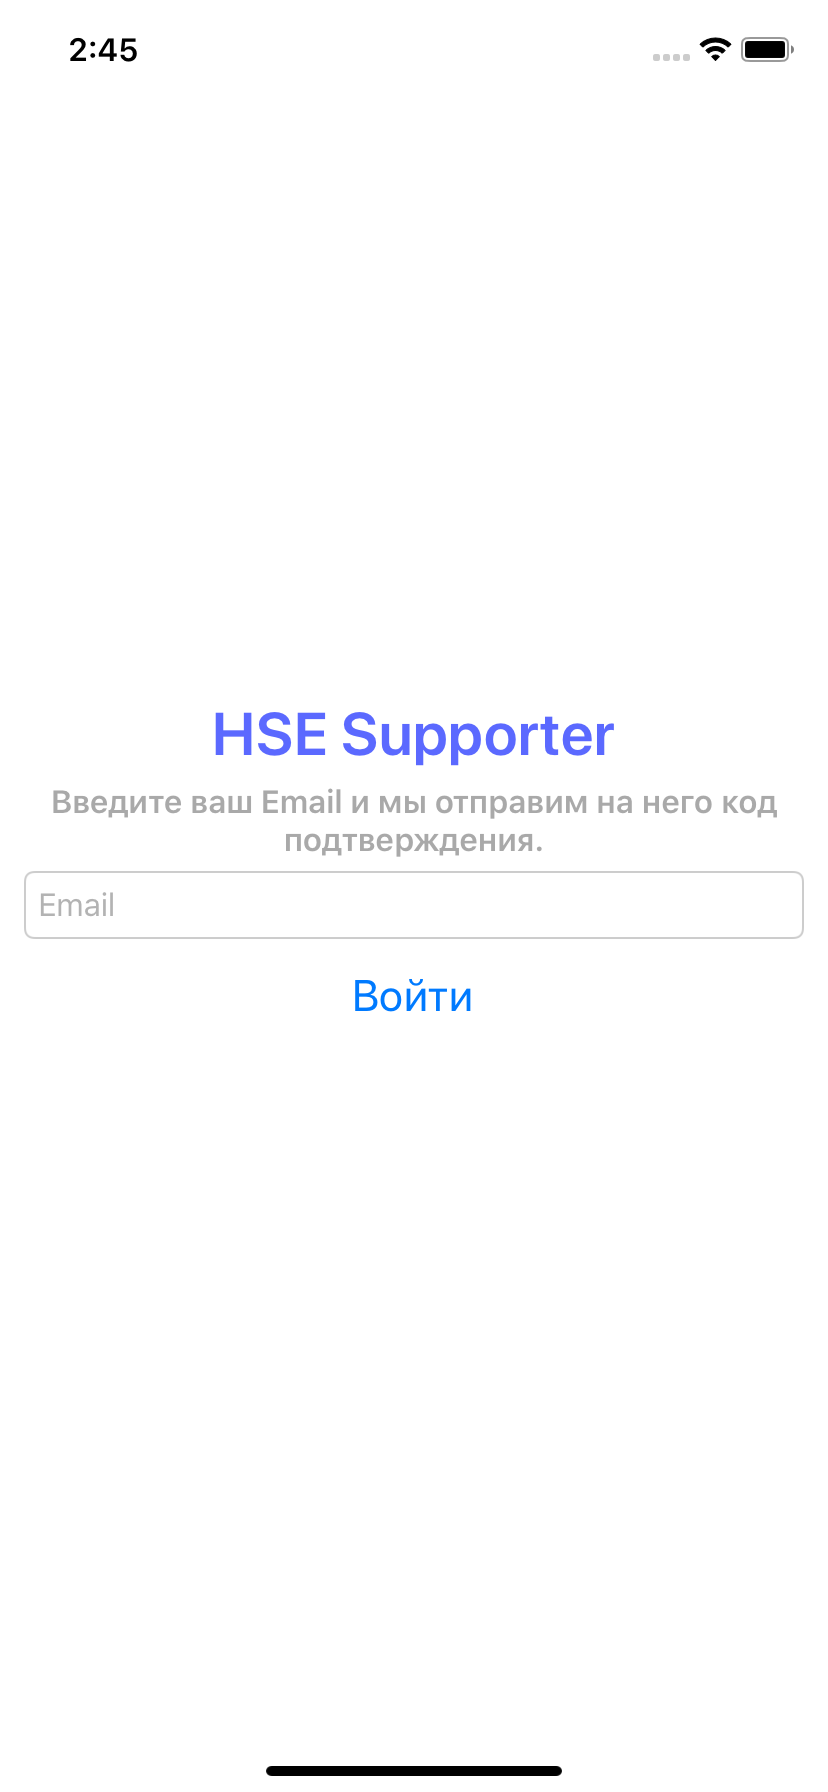
\includegraphics[width=0.4\linewidth]{images/login.png}}
            \caption{Экран авторизации}
            \label{fig:login}
        \end{figure}

        \newpage
        \item Для авторизации требуется сделать следующие действия:
        \begin{enumerate}
            \item Ввести Email в домене @hse.ru или @edu.hse.ru и нажать кнопку <<Войти>> (Рис.~\ref{ris:login_code});
            \item Ввести код подтверждения, который был отправлен на указанную почту и нажать кнопку <<Войти>>;
            \item Указать действительные персональные данные (Рис.~\ref{ris:personal_data}).
        \end{enumerate}
        \begin{figure}[h]
            \begin{center}
                \begin{minipage}[ht]{0.4\linewidth}
                    \frame{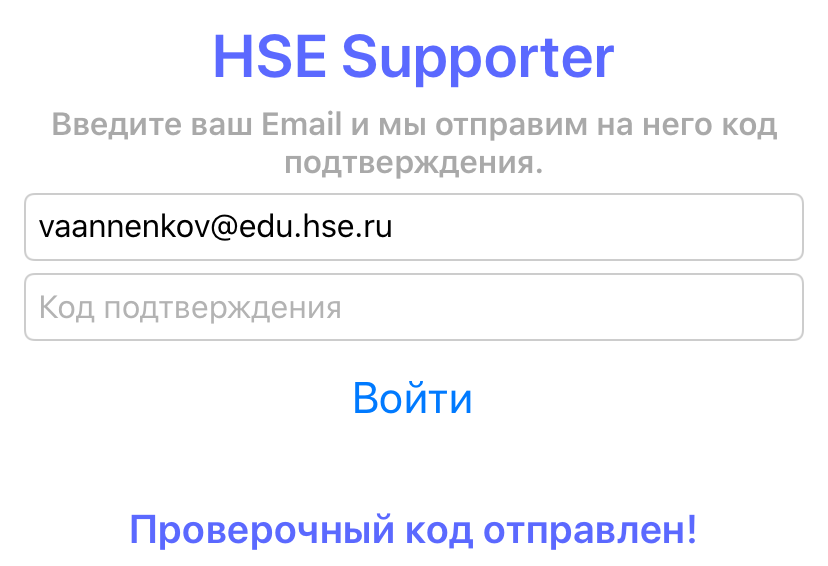
\includegraphics[width=1\linewidth]{images/login_code_success.png}}
                    \caption{После введения Email} %% подпись к рисунку
                    \label{ris:login_code} %% метка рисунка для ссылки на него
                \end{minipage}
                \hfill
                \begin{minipage}[ht]{0.4\linewidth}
                    \frame{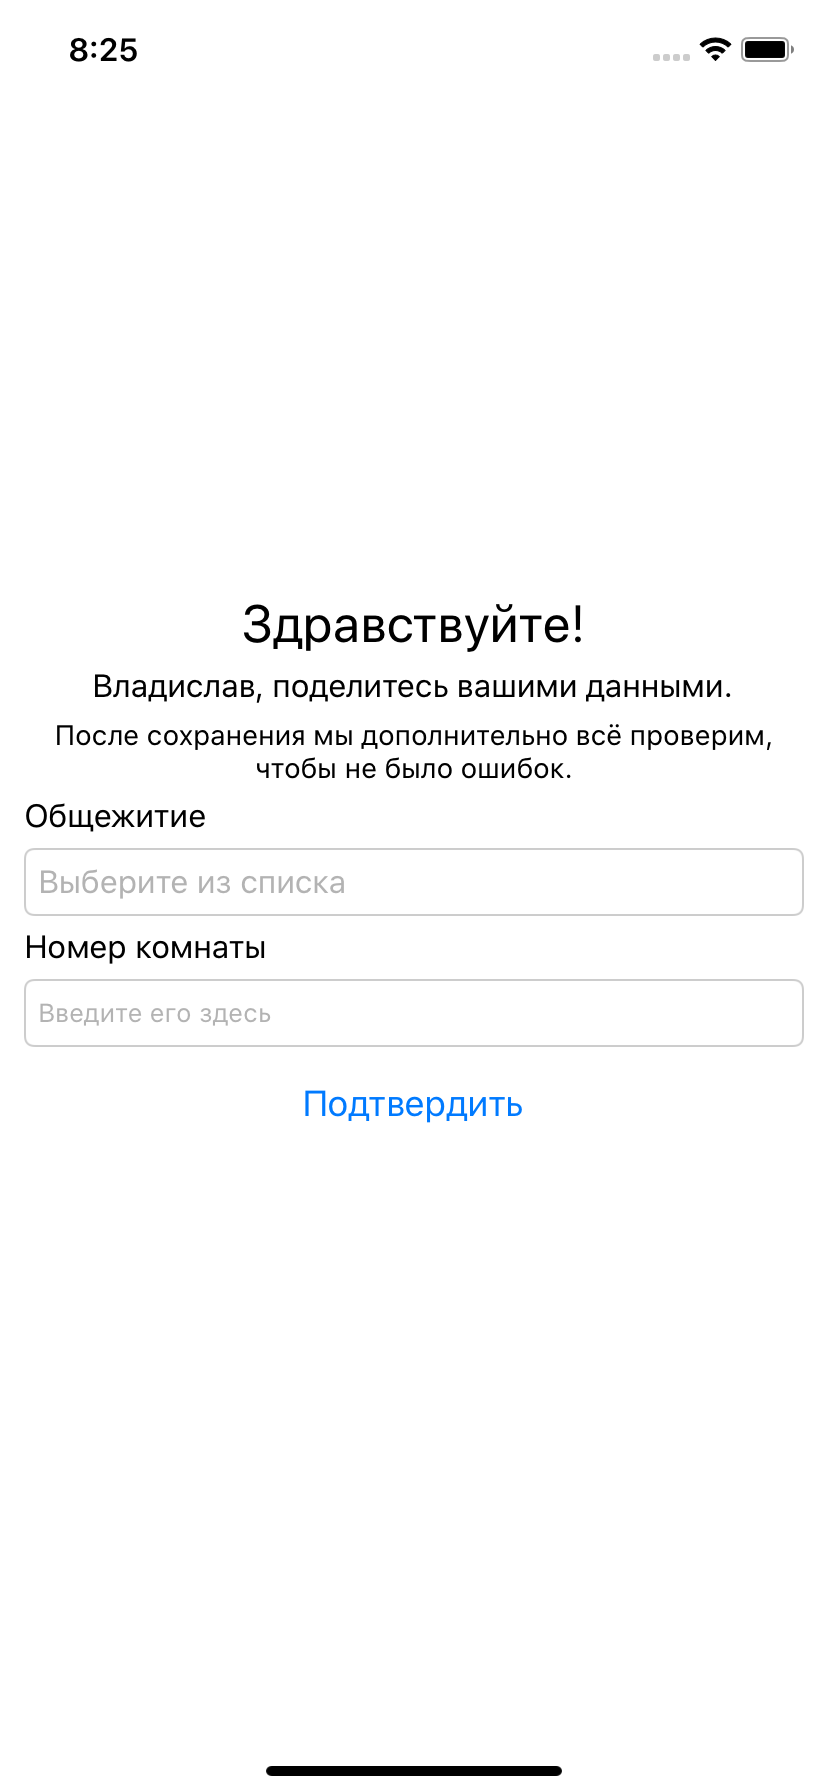
\includegraphics[width=1\linewidth]{images/wait_page.png}}
                    \caption{Ввод персональных данных}
                    \label{ris:personal_data}
                \end{minipage}
            \end{center}
        \end{figure}

        \item После успешной авторизации пользователь попадает на главный экран.
        Управление происходит через нижнюю панель (Рис.~\ref{fig:menu}), на которой располагаются кнопки:
        \begin{enumerate}[noitemsep]
            \item Главная;
            \item Обращения;
            \item Беседа;
            \item О приложении;
        \end{enumerate}
    \end{enumerate}

    \begin{figure}[ht]
        \centering
        \frame{
\includegraphics[width=1\linewidth]{images/menu.png}}
        \caption{Меню}
        \label{fig:menu}
    \end{figure}

    \clearpage

    \paragraph{Главная}

    \begin{enumerate}
        \item На главном экране (Рис.~\ref{ris:main_page}) располагаются новости общежития, важные уведомления вверху страницы,
        а также кнопка <<Профиль>> для редактирования профиля.
        \item Список новостей представляет из себя горизонтальную <<карусель>>, новости можно перелистывать движением пальца.
        \item На любую новость можно нажать, чтобы посмотреть более подробную информацию.
        \item Информацию главной страницы можно обновить, потянув страницу вверх до появления индикатора загрузки.

        \item При нажатии на кнопку <<Профиль>> появляется экран (Рис.~\ref{ris:profile_page}) со следующими полями:
        \begin{enumerate}[noitemsep]
            \item Имя;
            \item Фамилия;
            \item Общежитие;
            \item Комната.
        \end{enumerate}
        В каждое поле, кроме полей <<Имя>> и <<Фамилия>>, можно вносить изменения.
        \begin{figure}[ht]
            \begin{center}
                \begin{minipage}[h]{0.33\linewidth}
                    \frame{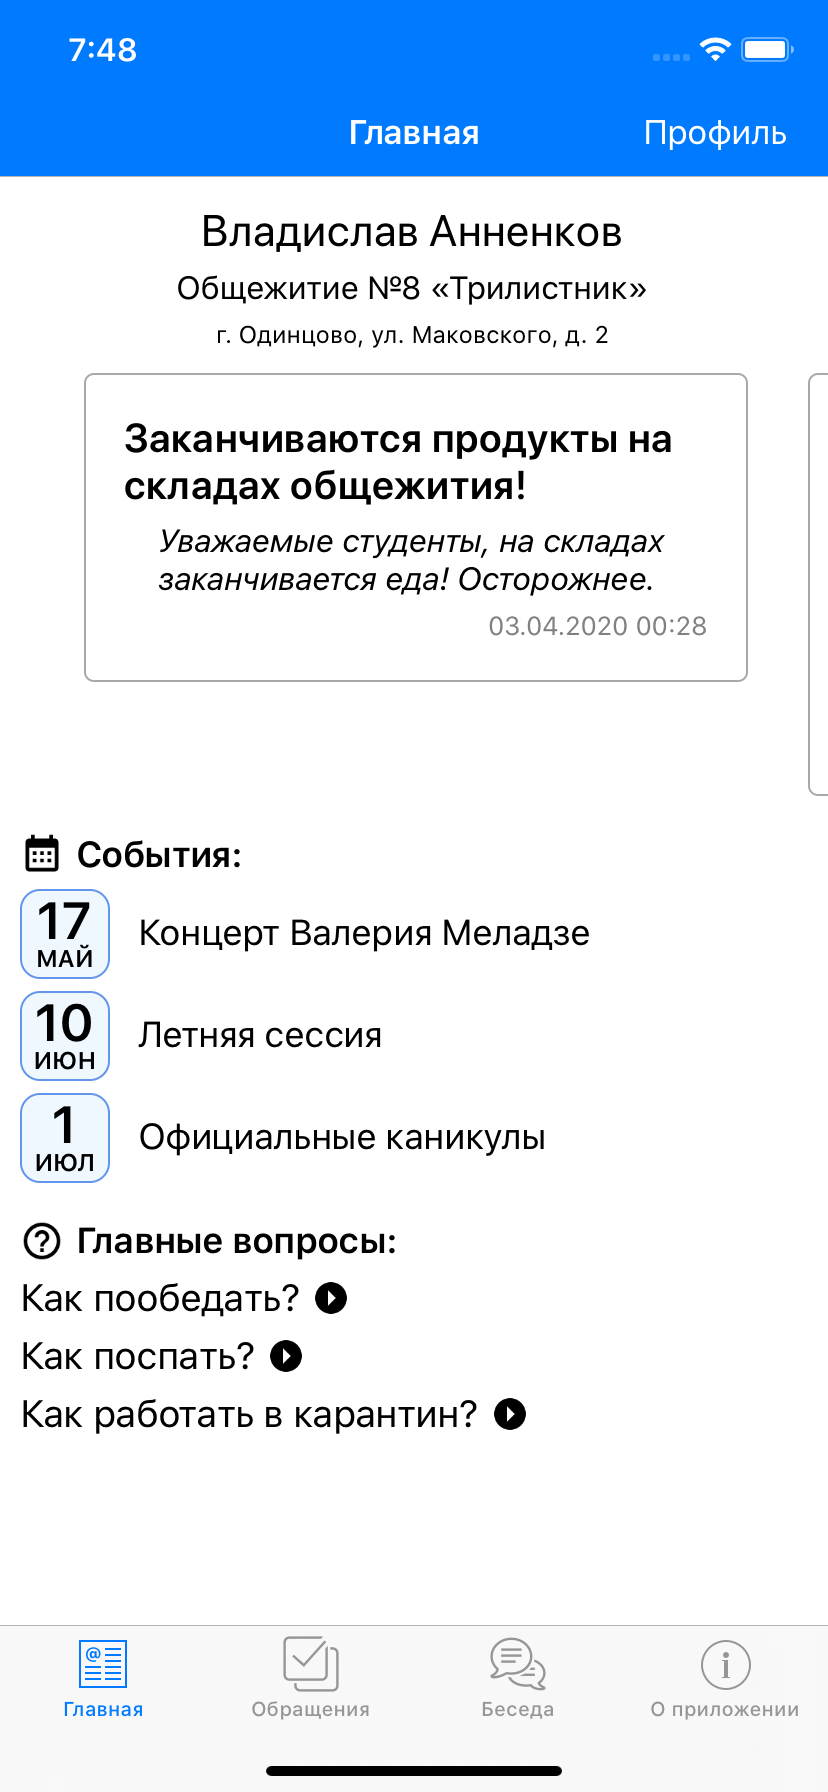
\includegraphics[width=1\linewidth]{images/main_page.png}}
                    \caption{Главный экран} %% подпись к рисунку
                    \label{ris:main_page} %% метка рисунка для ссылки на него
                \end{minipage}
                \hfill
                \begin{minipage}[h]{0.33\linewidth}
                    \frame{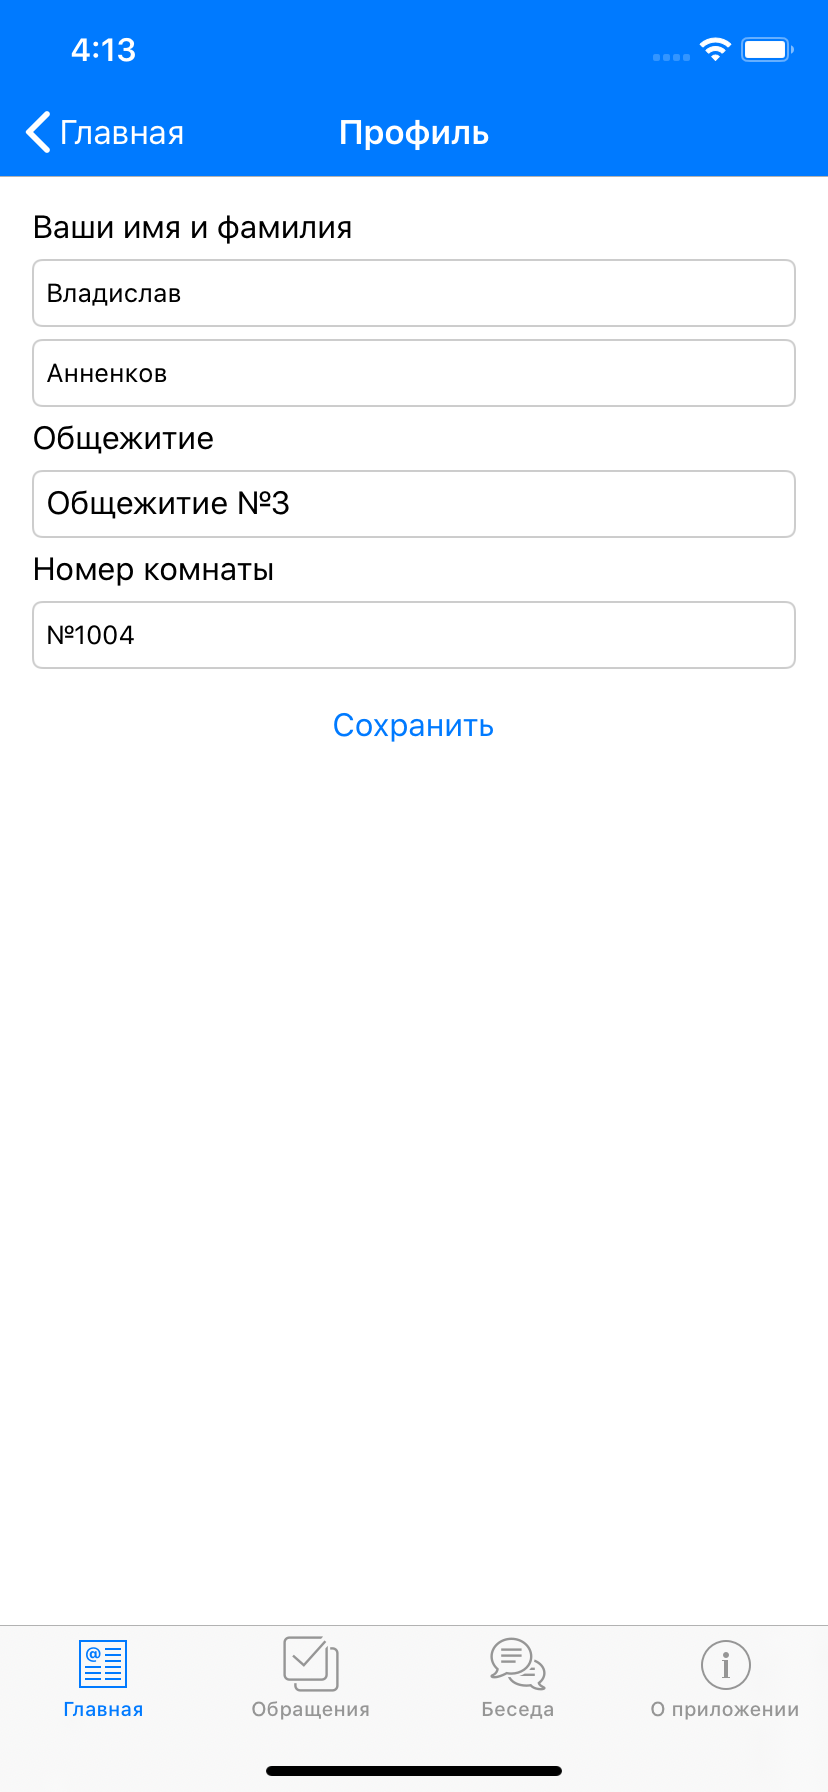
\includegraphics[width=1\linewidth]{images/profile_page.png}}
                    \caption{Профиль}
                    \label{ris:profile_page}
                \end{minipage}
            \end{center}
        \end{figure}

        \item После изменений требуется нажать на кнопку <<Сохранить>>.
        \item После сохранения изменений профиль пользователя попадает в очередь на модерацию введённых данных.

    \end{enumerate}

    \clearpage

    \paragraph{Обращения}

    \begin{figure}[ht]
        \begin{center}
            \begin{minipage}[h]{0.32\linewidth}
                \frame{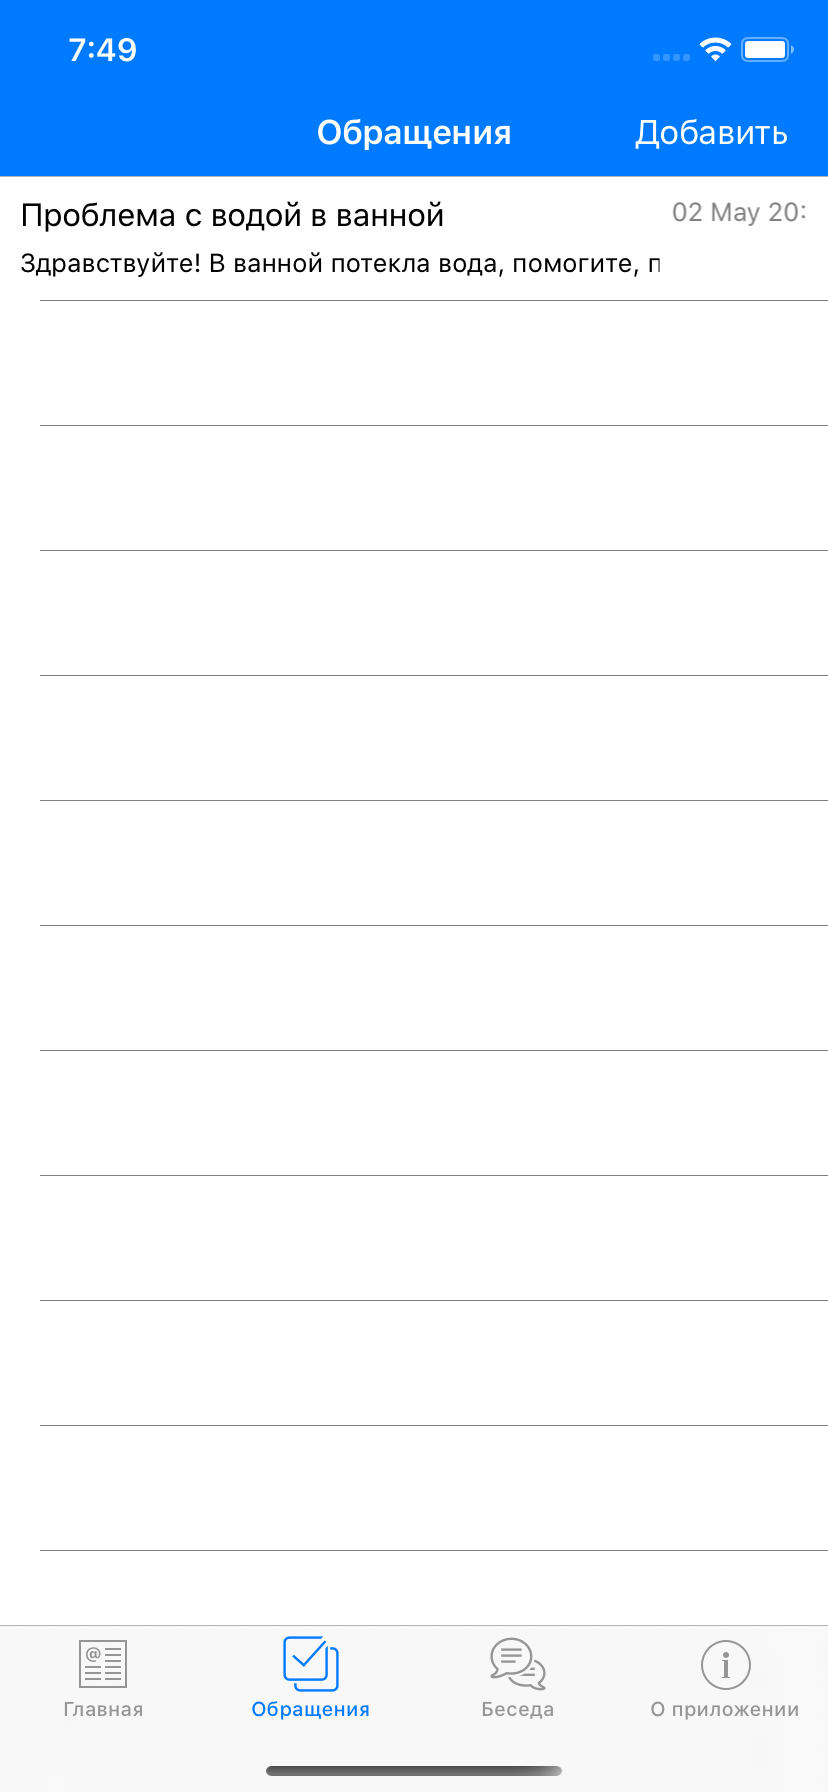
\includegraphics[width=1\linewidth]{images/problems_page.png}}
                \caption{Список обращений} %% подпись к рисунку
                \label{ris:problems} %% метка рисунка для ссылки на него
            \end{minipage}
            \hfill
            \begin{minipage}[h]{0.32\linewidth}
                \frame{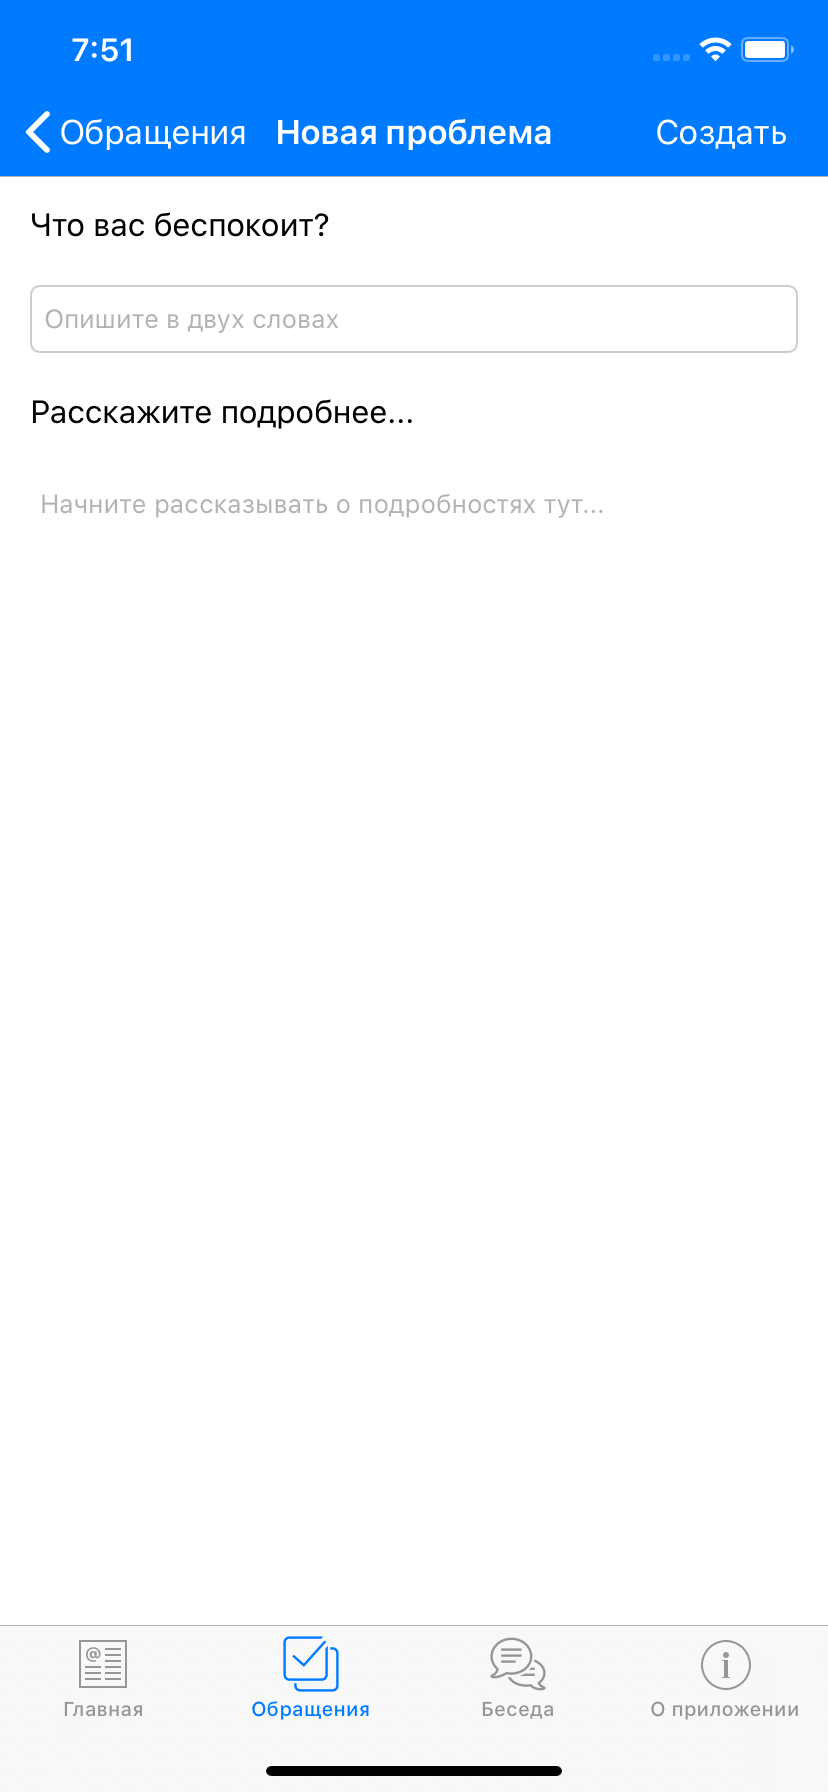
\includegraphics[width=1\linewidth]{images/new_problem_page.png}}
                \caption{Создание нового обращения}
                \label{ris:new_problem}
            \end{minipage}
            \hfill
            \begin{minipage}[h]{0.32\linewidth}
                \frame{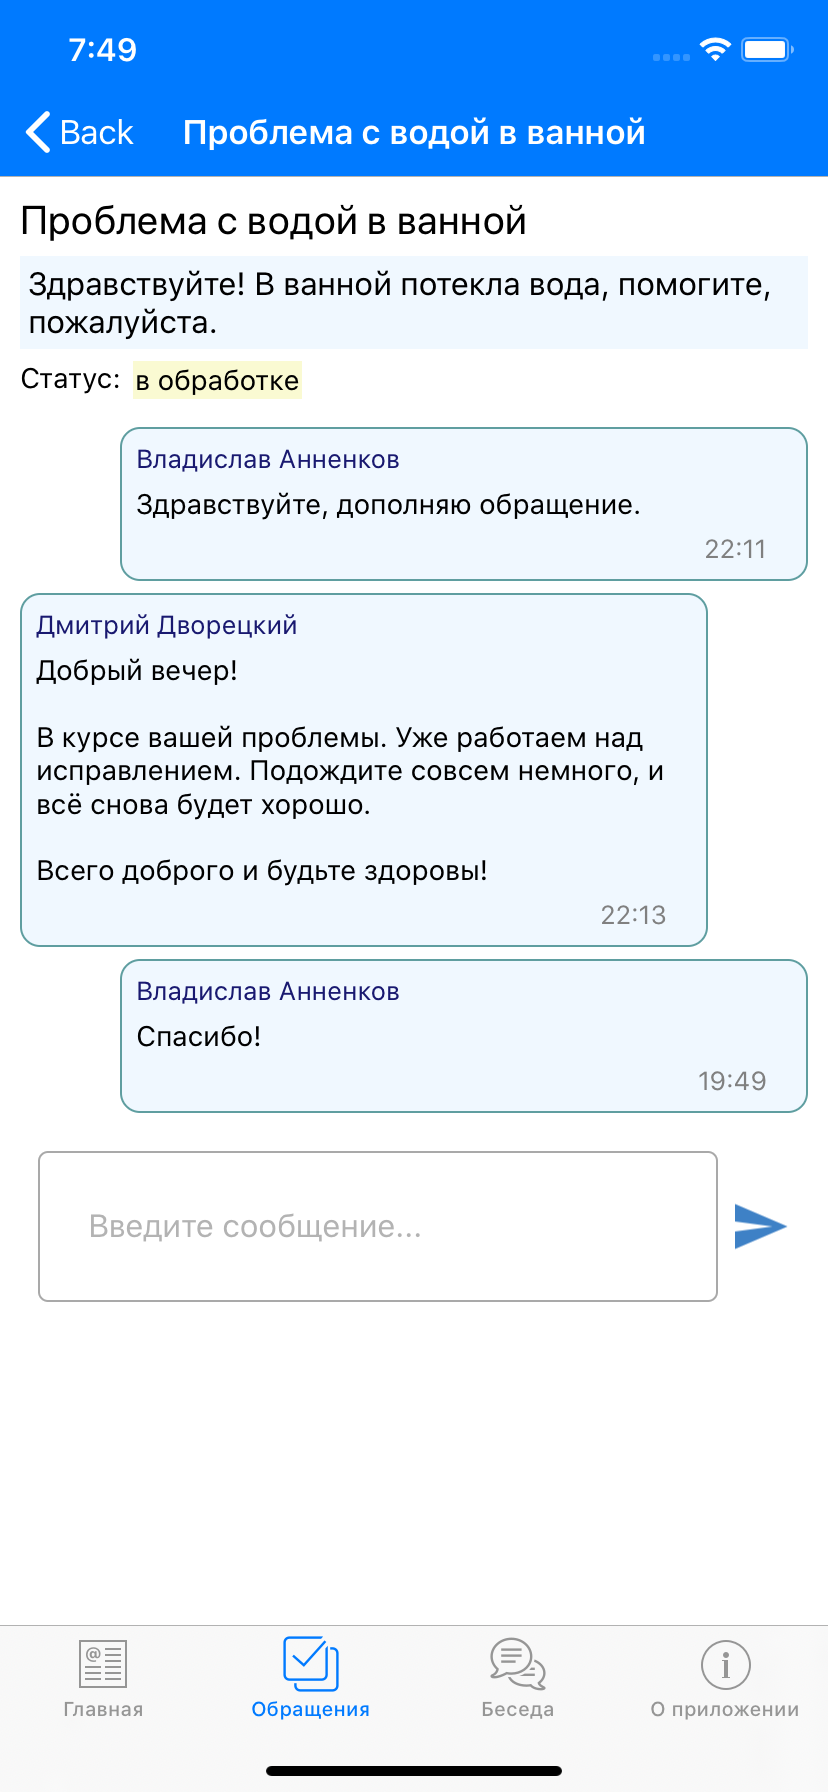
\includegraphics[width=1\linewidth]{images/problem_details_page.png}}
                \caption{Детальная информация обращения}
                \label{ris:problem_details}
            \end{minipage}
        \end{center}
    \end{figure}

    \begin{enumerate}
        \item На экране с обращениями (Рис.~\ref{ris:problems}) располагаются обращения, созданные пользователем.

        \item Обращение можно создать, нажав на кнопку <<Добавить>> и введя необходимые данные в соответствующие поля (Рис.~\ref{ris:new_problem}).

        \item После создания обращения оно появляется в списке обращений.
        \item Для просмотра более подробной информации можно нажать на обращение.
        \item На странице с подробной информацией обращения (Рис.~\ref{ris:problem_details}) находятся следующие элементы:
        \begin{enumerate}
            \item заголовок;
            \item подробное описание;
            \item статус обращения;
            \item дата создания;
            \item диалог пользователя с агентом поддержки;
        \end{enumerate}

        \item Для того, чтобы отправить сообщение в чат с агентом поддержки, требуется набрать текст
        в соответствующее поле, а затем нажать на значок с бумажным самолётиком.

        \item Для удаления обращения можно потянуть требуемое обращение влево, а затем нажать на красную кнопку <<Удалить>>.
    \end{enumerate}

    \clearpage

    \paragraph{Беседа}

    \begin{enumerate}
        \item Для просмотра списка сообщений беседы требуется открыть соответствующий экран (Рис.~\ref{fig:chat}), дополнительных действий не требуется.
        \begin{figure}[ht]
            \centering
            \frame{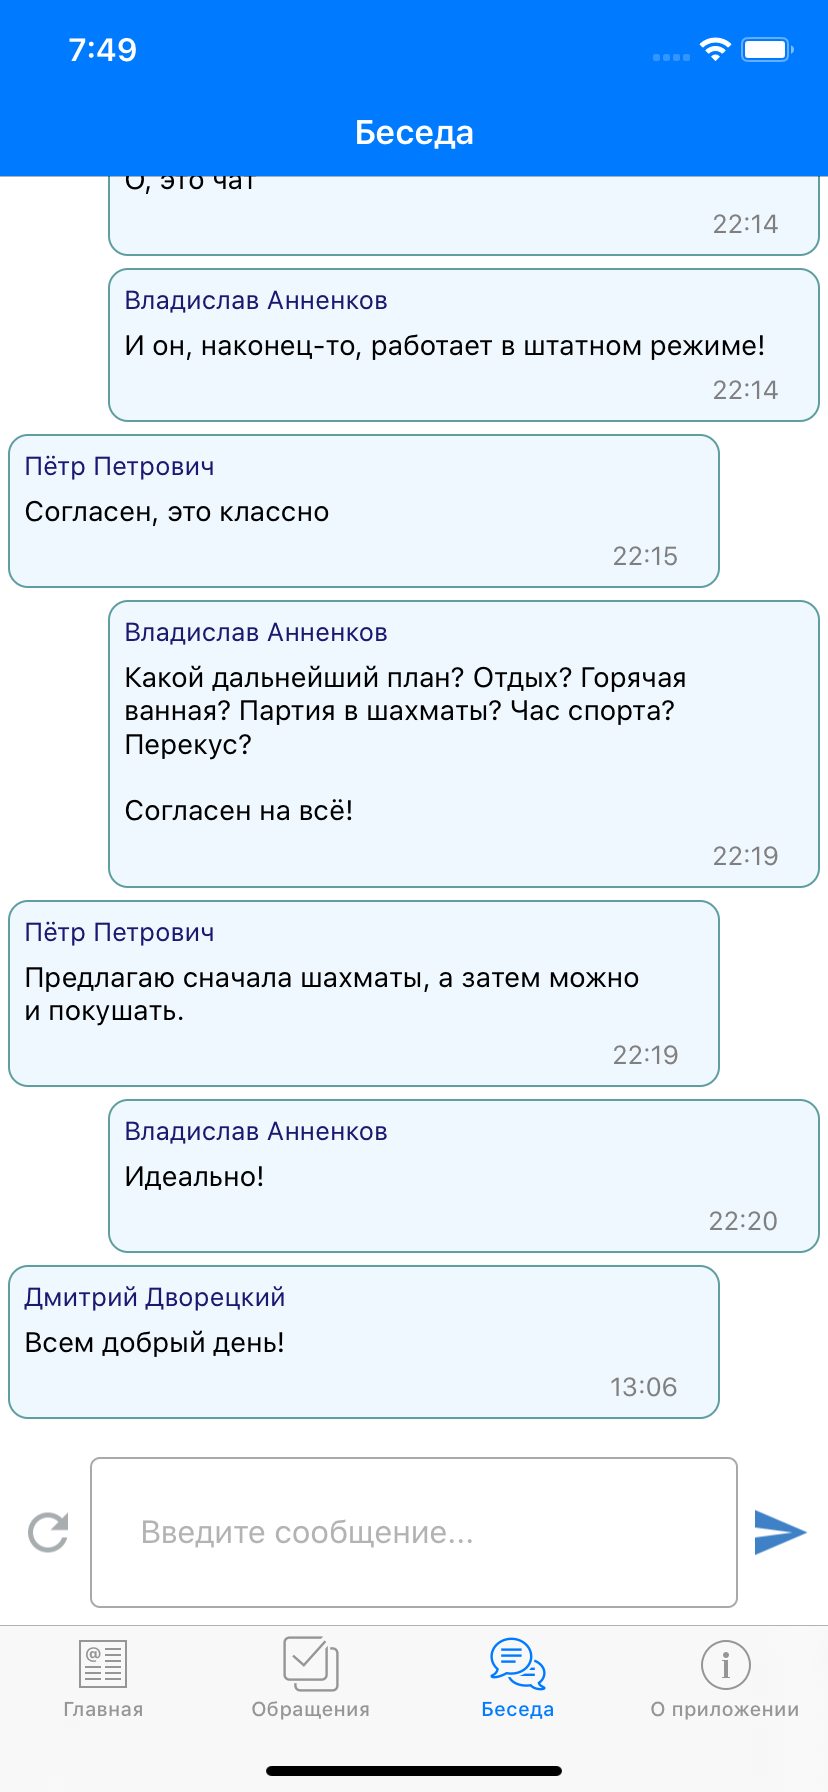
\includegraphics[width=0.3\linewidth]{images/chat_page.png}}
            \caption{Беседа общежития}
            \label{fig:chat}
        \end{figure}

        \item Всё взаимодействие с беседой происходит внутри определённого общежития. У каждого общежития свои беседы и они не пересекаются.
        \item Для отправки сообщения требуется ввести текст в соответствующее поле и нажать на кнопку с синим бумажным самолётиком.
        \item Для обновления беседы требуется нажать на кнопку с иконкой круговой стрелки.
    \end{enumerate}

    \clearpage

    \subsubsection{Описание интерфейса панели администрирования}

    \paragraph{Авторизация}

    Для авторизации (Рис.~\ref{ris:admin_login}) требуется заполнить поля <<Имя пользователя>> и <<Пароль>>.
    Данные для авторизации агенты поддержки получают от администратора системы.
    \begin{figure}[ht]
        \centering
        \frame{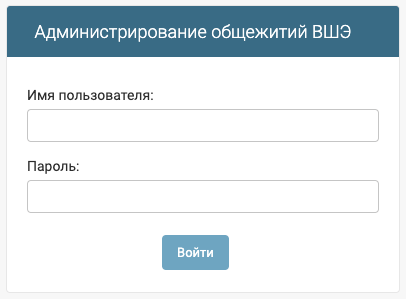
\includegraphics[width=0.7\linewidth]{images/admin_login.png}}
        \caption{Экран авторизации в панели администрирования}
        \label{ris:admin_login}
    \end{figure}

    \clearpage

    \paragraph{Главная страница}

    На главной странице панели администрирования (Рис.~\ref{ris:admin_main}) расположены следующие элементы:
    \begin{enumerate}
        \item Модели:
        \begin{enumerate}
            \item Обращения;
            \item Объявления;
            \item Профили;
            \item События;
            \item Сообщения.
        \end{enumerate}
        \item Последние действия — любые действия, которые производились над моделями;
        \item Вспомогательные кнопки в шапке сайта:
        \begin{enumerate}
            \item Открыть сайт — открывает главный сайт с методами REST API;
            \item Изменить пароль — позволяет изменить пароль текущего аккаунта;
            \item Выйти — позволяет выйти из аккаунта.
        \end{enumerate}
    \end{enumerate}
    \begin{figure}[ht]
        \centering
        \frame{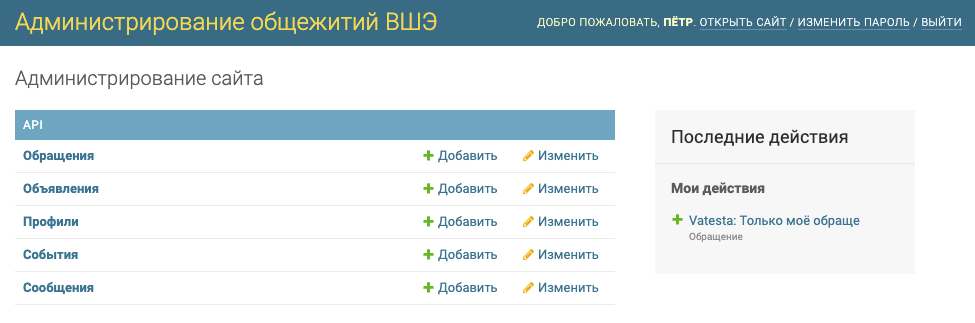
\includegraphics[width=1\linewidth]{images/admin_main.png}}
        \caption{Главный экран панели администрирования}
        \label{ris:admin_main}
    \end{figure}

    \clearpage

    \paragraph{Список моделей определённого типа}

    Для просмотра списка моделей определённого типа, достаточно нажать на элемент с именем типа требуемой модели.
    Для примера откроем список моделей типа <<Профиль>>, нажав на элемент <<Профили>>.
    На экране списка моделей (Рис.~\ref{ris:admin_model_list}) отображаются все модели, относящиеся к выбранному типу, блок поиска сверху, а также блок фильтрации справа.

    При нажатии на параметры блока фильтрации список моделей будет обновляться в реальном времени.
    Например, если нажать на параметр <<Подтверждён ли администратором>> — <<Да>>, то будут отображаться
    все модели, которые соответствуют данному фильтру.

    Каждую модель можно отметить галочкой.
    Для отмеченных галочкой моделей можно совершить действие из пункта <<Действие>>.
    В данном пункте находится единственное действие — <<Удалить>>.
    Это позволяет быстро удалить несколько моделей одновременно.
    \begin{figure}[ht]
        \centering
        \frame{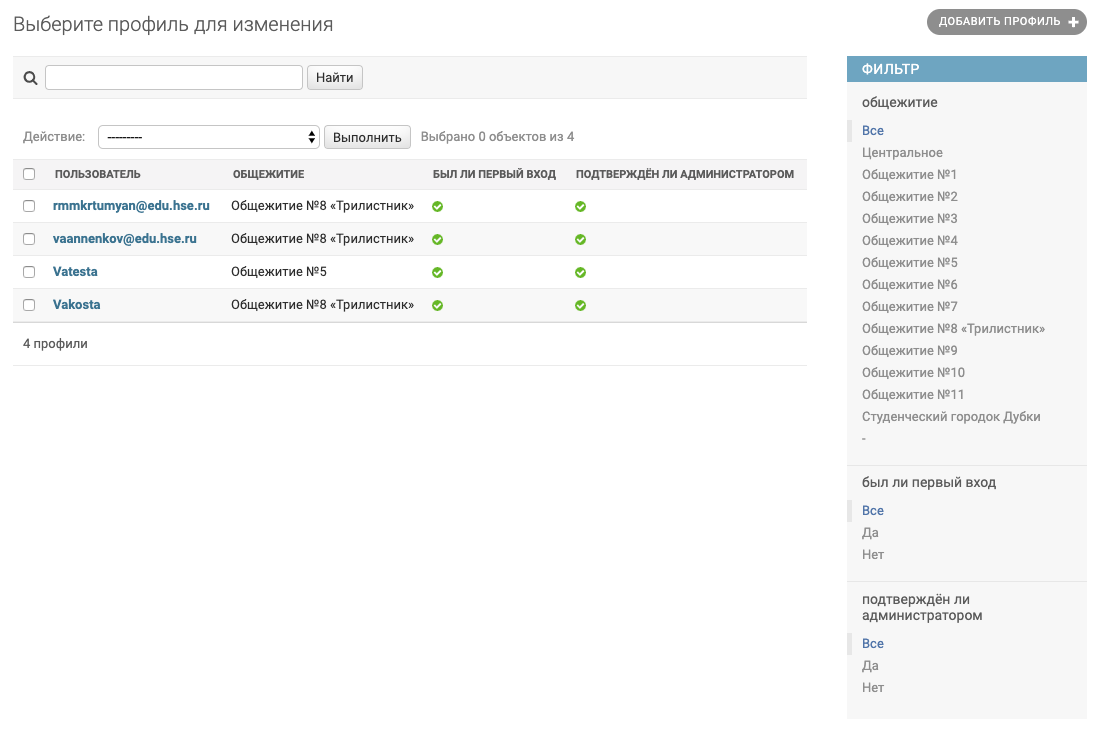
\includegraphics[width=1\linewidth]{images/admin_model_list.png}}
        \caption{Экран со списком моделей типа <<Профиль>>}
        \label{ris:admin_model_list}
    \end{figure}

    Для каждого типа моделей предусмотрены свои поля и фильтры, поэтому данная страница может отличаться для других типов моделей.

    \clearpage

    \paragraph{Редактирование модели}

    На экране редактирования модели (Рис.~\ref{ris:admin_model_edit}) каждая модель содержит свой набор полей.
    Вот типы полей, которые могут встречаться при редактировании моделей:
    \begin{enumerate}
        \item Короткое текстовое поле — текстовое поле, рассчитанное на небольшое количество текста;
        \item Большое текстовое поле — текстовое поле, предназначенное для больших объёмов текста;
        \item Поле-список — поле с возможностью выбора одного из заранее заданных значений;
        \item Логическое поле — поле с двумя значениями: <<да>> или <<нет>>;
        \item Поле с датой и временем — поле, которое содержит данные о дате и времени;
        \item Ссылочное поле — поле, которое ссылается на другой объект (этой же или сторонней модели).
    \end{enumerate}

    Изменения можно сохранить, нажав на одну из соответствующих кнопок.
    Модель можно удалить, нажав на кнопку <<Удалить>>.
    \begin{figure}[ht]
        \centering
        \frame{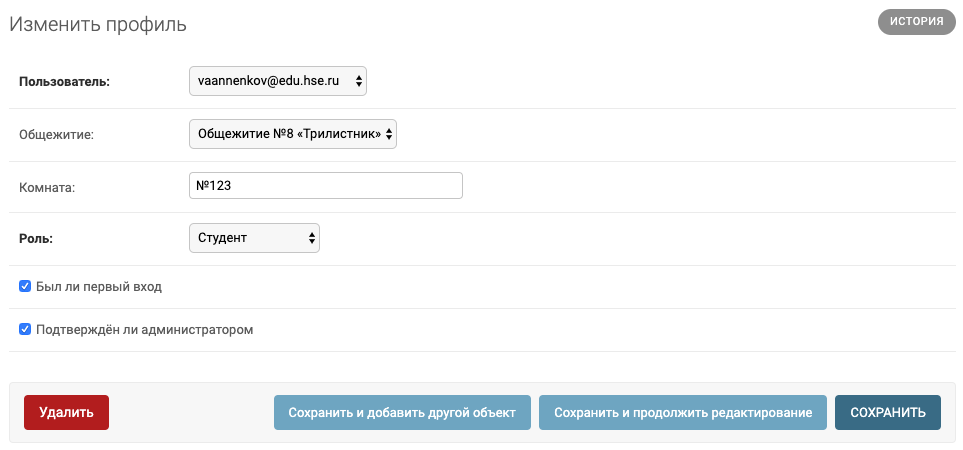
\includegraphics[width=1\linewidth]{images/admin_model_edit.png}}
        \caption{Экран редактирования модели}
        \label{ris:admin_model_edit}
    \end{figure}

    \clearpage


    \section{Источники, использованные при разработке}

    \begin{enumerate}
        \item ГОСТ 19.101-77 Виды программ и программных документов. // Единая система программной документации. – М.: ИПК Издательство стандартов, 2001.
        \item ГОСТ 19.102-77 Стадии разработки. // Единая система программной документации. – М.: ИПК Издательство стандартов, 2001.
        \item ГОСТ 19.103-77 Обозначения программ и программных документов. // Единая система программной документации. – М.: ИПК Издательство стандартов, 2001
        \item ГОСТ 19.104-78 Основные надписи. // Единая система программной документации. – М.: ИПК Издательство стандартов, 2001.
        \item ГОСТ 19.105-78 Общие требования к программным документам. // Единая система программной документации. – М.: ИПК Издательство стандартов, 2001.
        \item ГОСТ 19.106-78 Требования к программным документам, выполненным печатным способом. // Единая система программной документации. – М.: ИПК Издательство стандартов, 2001
        \item ГОСТ 19.404-79 Пояснительная записка. Требования к содержанию и оформлению. // Единая система программной документации. – М.: ИПК Издательство стандартов, 2001.
        \item LMS [Электронный ресурс] URL: \url{https://lms.hse.ru/} (Дата обращения: 15.05.2020, режим доступа: свободный)
        \item РУЗ [Электронный ресурс] URL: \url{https://ruz.hse.ru/} (Дата обращения: 15.05.2020, режим доступа: свободный)
        \item GitHub [Электронный ресурс] URL: \url{https://github.com/} (Дата обращения: 15.05.2020, режим доступа: свободный)
        \item Документация Microsoft [Электронный справочник] URL: \url{https://docs.microsoft.com/ru-ru/} (Дата обращения: 15.05.2020, режим доступа: свободный)
        \item Документация Python [Электронный справочник] URL: \url{https://docs.python.org/3/} (Дата обращения: 15.05.2020, режим доступа: свободный)
        \item StackOverflow [Электронный ресурс] URL: \url{https://stackoverflow.com/} (Дата обращения: 15.05.2020, режим доступа: свободный)
        \item Документация библиотеки <<Refit>> [Электронный справочник] URL: \url{https://reactiveui.github.io/refit/} (Дата обращения: 15.05.2020, режим доступа: свободный)
        \item Документация фреймворка <<Django REST framework>> [Электронный справочник] URL: \url{https://www.django-rest-framework.org/} (Дата обращения: 15.05.2020, режим доступа: свободный)
    \end{enumerate}


    \registrationList

\end{document}
